\documentclass[12pt,number]{IC_fyp}
\usepackage{a4wide,amsmath,amssymb,epsfig,authordate1-4}
\usepackage{float}
\floatstyle{plaintop}
\restylefloat{table}
\usepackage[small]{caption}
\usepackage[tight]{subfigure}
\bibliographystyle{authordate2}

%% Don't edit above this line, unless you know what you are doing %% 

\begin{document}

\title{Paper title here}

\author{Romeo Beckham}

\address{Department of Civil and Environmental Engineering\\
  Imperial College London}

\begin{frontmatter}
  
\begin{abstract}

Write your abstract here, up to 200 words.

\end{abstract}

\end{frontmatter}

\section{Introduction}
\label{sec:intro}

In \LaTeX, there are lots of advantages: cross referencing of figures,
tables and equations can be purely symbolic, as can citing
references. Once this is appreciated, this will allow you to focus
purely on the report text. The rules of the Word Template are
automatically followed. Figure \ref{fig:example}
\begin{figure}[htbp]
	\centerline{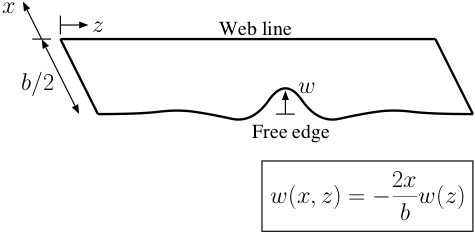
\psfig{figure=wdef_linear,width=6cm}}
%  \centerline{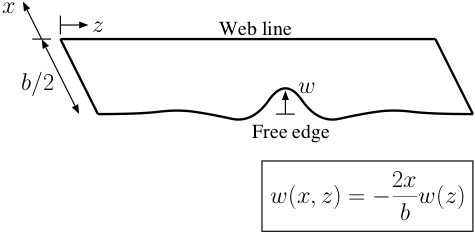
\psfig{figure=wdef_linear.ps,width=100mm}}
  \caption{Example diagram in EPS format. Caption is centred and goes
    below diagram.}
  \label{fig:example}
\end{figure}
shows an example diagram taken from a recent paper by Wadee and Gardner
\shortcite{Wadee_ltblocal_2012}. Table \ref{tab:example}
\begin{table}[htbp]
  \begin{center}    
  \begin{tabular}{|c|c|c|}
    \hline
    Experiment & $P_l^\mathrm{C}$ (kN) & $P_o^\mathrm{C}$ (kN)\\
    \hline
    1 & 20.0 & 15.0 \\
    2 & 15.0 & 20.0 \\
    3 & 18.5 & 18.5 \\
    \hline
  \end{tabular}
  \end{center}
  \caption{This is an example of a table. Use the ``tabular''
    environment to insert the actual table. The caption needs to be
    centred as before but, unlike figures, they should be above the table.}
\label{tab:example}
\end{table}
shows an example of a table listing a set of example experimental data
that gives information on a series of experiments. Equations are
similarly numbered:
\begin{equation}
  F = m\ddot{x},
  \label{eq:Newton2nd}
\end{equation}
and should be punctuated. Equation (\ref{eq:Newton2nd}) shows a
reference to Newton's 2nd law of motion for constant mass $m$. When
referred to in the text, Equation numbers should always be listed
between parentheses as shown in the previous sentence.

\section{Second Section}
\label{sec:2nd}

More text here.

\subsection{Sub-Section}

Even more text here. Figures and tables can be inserted as before, but
here is some text to demonstrate a new paragraph. Leave a line space
in the text file for a new paragraph.

This is a new paragraph here.

\subsubsection{Sub-Sub-Section}

Make sure that you are clear and concise in your presentation of your
paper, it is a critical skill that will be used throughout your career.

References are to be cited in the Harvard style: an excellent package
in the bibliography creating program BibTeX is ``authordate''. For
example, we saw Wadee and Gardner \shortcite{Wadee_ltblocal_2012}
being cited above. They wrote a seminal paper based on previous work
\cite{vk_sechler_donnell_1932,cherry_ltb_local_1960,nondyn}. Once
\LaTeX~is run, the cited references appear where the
\begin{verbatim}
\bibliography{}
\end{verbatim}
command appears in the text file. A recommendation is to use the freely
available software ``Jabref'' to manage references. Note that with the
style ``authordate'' the citations with three or more authors are
automatically abbreviated to ``Author \emph{et al}''. Should there be
more than one reference with an identical citation, for example
\cite{MAW_jsg}, the year of the citation will be augmented
automatically by a letter (\emph{e.g.}\ a, b, c, and so on).

\section{Third Section}

\section{Fourth Section}

\section{Fifth Section}

\section{Concluding Remarks}

This does not have to the 6th section, although in this example it
is. Please write clear and concise conclusions.

\section*{Acknowledgement}

You may wish to acknowledge your supervisor somewhere here\ldots

\bibliography{refs}

\end{document}
